\section{Rastreabilidade}
	A rastreabilidade auxilia a engenharia de requisitos no controle dos requisitos, elementos de modelagem e outros artefatos do processo de software. Por meio dela, é possivel obter visualizar de onde surgiu tal requisito, quais são suas dependências e ainda quais deles serão afetados quando houver algum tipo de mudança.\\

	\begin{figure}[!htb]
		\centering
		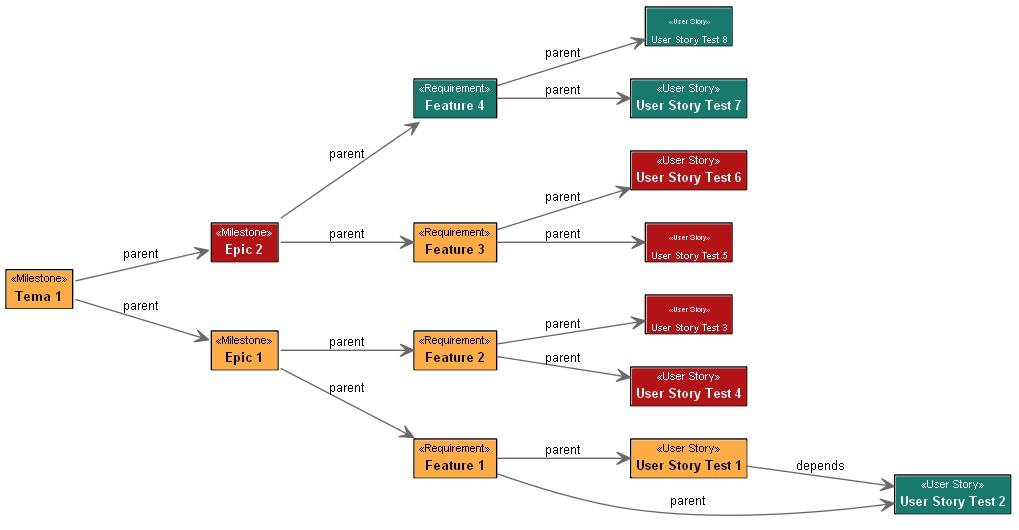
\includegraphics[width = \textwidth]{imagens/rastreabilidade.jpg}
		\caption{exemplo de rastreabilidade vertical e horizontal}
		\label{imagem}
	\end{figure}

	No desenvolver deste projeto iremos utilizar dois tipos de rastreabildade, a vertical e a horizontal.
	
	\subsection{Rastreabilidade Vertical}
	A rastreabilidade vertical será utilizada no projeto para identificar a origem dos requisitos, ela está presente nas relações de um nível de abstração e outro.\\

	\begin{landscape}
	\begin{figure}[!htb]
		\centering
		\vspace*{2.5cm}
		\hspace*{-1cm}
		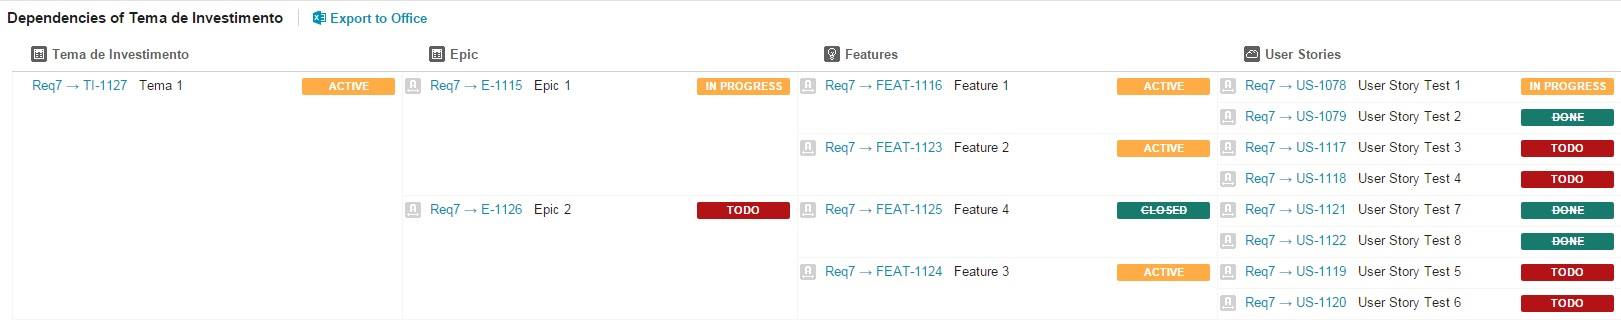
\includegraphics[width = 1.5\textwidth, height = 0.5\textheight]{imagens/rastreabilidade_vertical.jpg}
		\caption{exemplo de rastreabilidade vertical de tema de investimento à histórias de usuário.}
		\label{imagem}
	\end{figure}
	\end{landscape}

	\subsection{Rastreabilidade Horizontal}
	A rastreabilidade horizontal será utilizada no projeto para identificar as dependencias entre um requisito e outro de um mesmo nível de abstração.

	\begin{figure}[!htb]
		\centering
		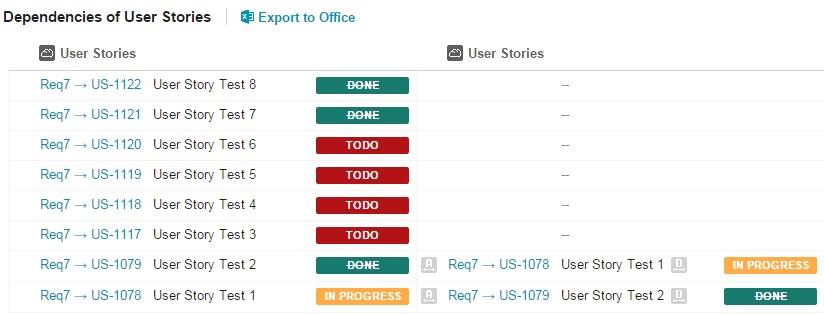
\includegraphics[width = \textwidth]{imagens/rastreabilidade_horizontal.jpg}
		\caption{exemplo de rastreabilidade horizontal entre histórias de usuário.}
		\label{imagem}
	\end{figure}
